\documentclass[a4paper,12pt]{article}
\usepackage{times}
\usepackage[francais]{babel}
\usepackage[utf8x]{inputenc}
\usepackage[T1]{fontenc}
\usepackage{amsmath}
\usepackage{amssymb}
\usepackage{graphicx}
\usepackage{pdfpages}
\usepackage{pdflscape}
\usepackage{listings}
\usepackage{longtable}
\usepackage{float}

\lstset{literate=
{é}{{\'e}}1
{è}{{\`e}}1
{ê}{{\^e}}1
{à}{{\`a}}1
{â}{{\^a}}1
}
\lstset{language=C++,
                basicstyle=\footnotesize,
                keywordstyle=\footnotesize\color{blue},
                otherkeywords={override,nullptr}
}
\definecolor{orange}{rgb}{0.8,0.4,0.0}
\definecolor{darkblue}{rgb}{0.0,0.0,0.6}
\definecolor{cyan}{rgb}{0.0,0.6,0.6}
\lstdefinelanguage{JSON}
{
  basicstyle=\normalsize,
  columns=fullflexible,
  showstringspaces=false,
  commentstyle=\color{gray}\upshape,
  morestring=[b]",
  morestring=[s]{>}{<},
  morecomment=[s]{<?}{?>},
  stringstyle=\color{orange},
  identifierstyle=\color{darkblue},
  keywordstyle=\color{blue},
  morekeywords={string,number,array,object}% list your attributes here
}

\sloppy

\setlength{\topmargin}{0cm}
\setlength{\headsep}{0.in}
\setlength{\headheight}{0.in}
\setlength{\evensidemargin}{0cm}
\setlength{\oddsidemargin}{-1cm}
\textwidth 18cm
\textheight 25cm

\begin{document}

\thispagestyle{empty}

\begin{titlepage}

\vspace*{2cm}

\begin{center}\textbf{\Huge Projet Logiciel Transversal}\end{center}{\Large \par}

\begin{center}\textbf{\large Mohamed KHLIFI et Ihsen OUERGHI}\end{center}{\large \par}

\vspace{2cm}

%\begin{figure}[h]
%\begin{center}
%\includegraphics[width=\textwidth]{exemple.png}
%\caption{\label{pacmangame}Exemple du jeu}
%\end{center}
%\end{figure}

\clearpage

{\small
\tableofcontents
}

\end{titlepage}

\clearpage
\section{Présentation Générale}

\subsection{Archétype}

\vspace{1\baselineskip}


Le jeu que  nous souhaitons réaliser consiste en une opposition entre 2 joueurs dans la conquête d’une map. Notre jeu s’appuie ainsi sur les archétypes des jeux Total War et Civilization. 

Au départ les deux joueurs se voient confier un nombre égal de ressources et une ville, le reste de la map restant caché pour l'instant. Dès lors, les deux joueurs vont devoir explorer la map, par l'intermédiare d'un type de joueur (nommé explorateur), se développer et conqérir de nouveaux territoires. Des combats peuvent survenir pour la conquête d'une ville, ceux-ci seront simulés et donneront lieu à un vainqueur qui remportera la ville.

Le jeu se finit lorsque l'un des joueurs conquièrent toute la map.
\\

Notre jeu mêlera donc gestion/expansion de territoire, gestion de matières premières et gestion de ressources humaines.
Le jeu comporte une map principale découpée en plusieurs villes. Au départ celles-ci sont inhabitées et chaque joueur peut les coloniser. Concernant les personnages, nous commencerons avec deux types différents : les explorateurs et les soldatss. Les explorateurs servent à colonier des villes pour pouvoir les contrôler. Les soldats servent aux combats et déterminent en bonne partie l'issue de ceux-ci.


\subsection{Règles du jeu}

\vspace{1\baselineskip}


Une ville possède deux états : inhabitée ou colonisée. 

Une ville ne peut être colonisée que par des explorateurs.

Chaque ville possède deux notes : défense et fertilité. La note de défense est conditionnée par le nombre de soldats et par les fortifications construites. 

Chaque joueur possède deux ressources : la nourriture et l'or.
Si une ville est déjà colonisée par l'adversaire, il faut l'attaquer pour la conquérir.

Les combats sont simulés et prennent en compte l'armée qui attaque d'un côté et la note de la ville et l'armée qui défend de l'autre.
\\

Les bâtiments disponibles sont : \begin{itemize}

\item Fermes et mines pour les ressources

\item Caserne et fortifications pour produire les soldats et la note de défense

\item Hôtel de ville pour produire les explorateurs

\end{itemize}


\subsection{Ressources}

\vspace{1\baselineskip}


Pour les ressources nous avons trouvé pour démarrer un tileset minimaliste mais largement suffisant pour réaliser ce que nous avons en tête simplement. Il a été ajouté au dossier res du projet.
\\

\begin{figure}[H]
\begin{center}
  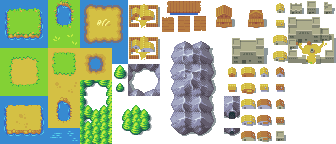
\includegraphics[width=0.7\textwidth]{images/tileset.png}
  \caption{Tileset pour la map}
 \end{center}

\end{figure}

Nous avons aussi besoin de sprites représentant les armées, pour cela nous avons trouvé en ligne un éditeur de personnages.

\begin{figure}[H]
\begin{center}
  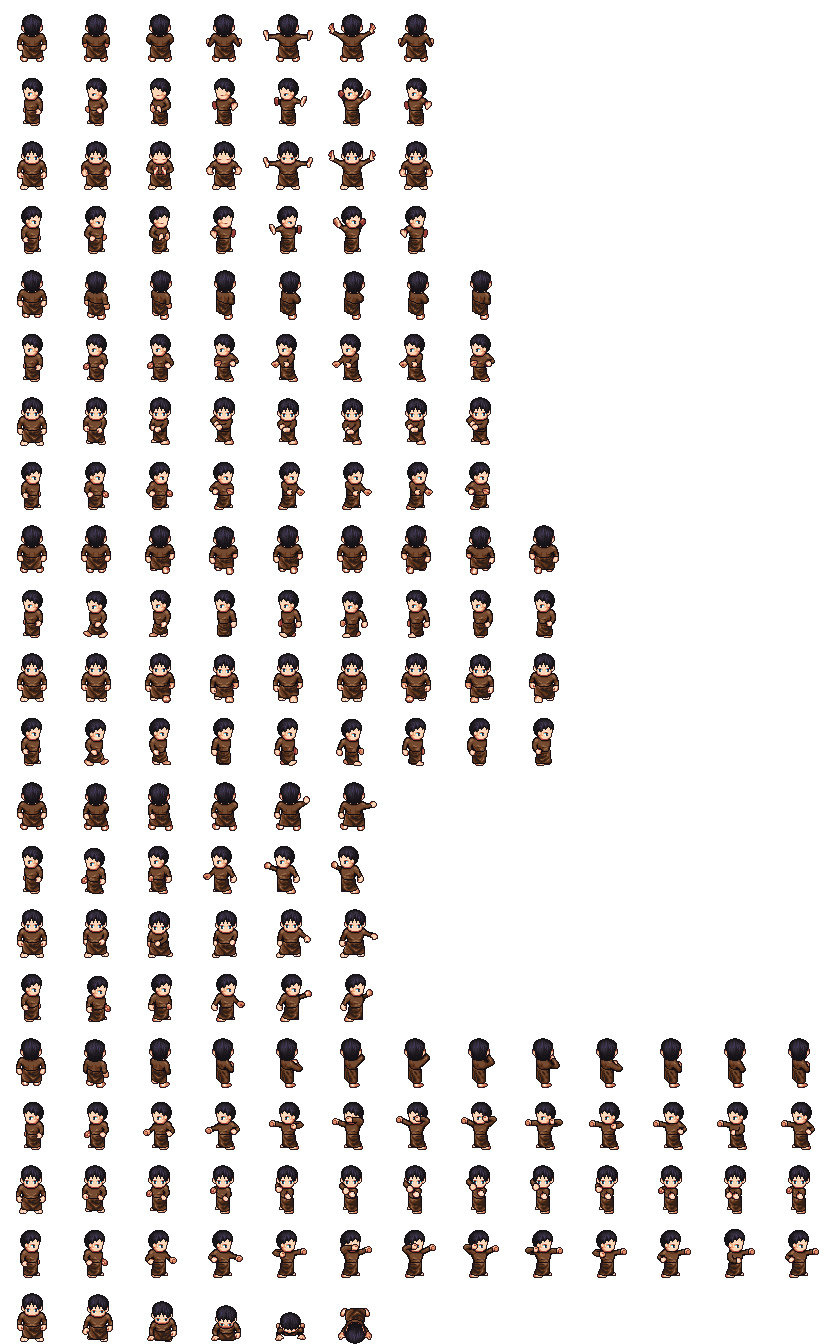
\includegraphics[width=0.7\textwidth]{images/sprite.png}
  \caption{Sprites pour les personnages}
 \end{center}

\end{figure}

Bien sur certaines animations du spritesheet ne seront pas utilisés.



%
%\begin{landscape}
%\begin{figure}[p]
%\includegraphics[width=0.9\paperheight]{module.pdf}
%\caption{\label{uml:module}Diagramme des classes pour la modularisation.} 
%\end{figure}
%\end{landscape}

\end{document}